\documentclass[aspectratio=169, table]{beamer}

\usepackage{listings}
\usepackage{tikz}
\usetikzlibrary{ fit, shapes.geometric, arrows.meta, positioning}
\usepackage{array}
\usepackage{float}
\usepackage{colortbl} 

\lstdefinestyle{RustStyle}{
	language=Java,
	morekeywords={println, Ok, async, fn, main, use, let, mut},
	basicstyle=\ttfamily\scriptsize,
	keywordstyle=\color{blue},
	commentstyle=\color{gray},
	stringstyle=\color{red},
	breaklines=true,
	showstringspaces=false,
	tabsize=2,
	captionpos=b,
	numbers=left,
	numberstyle=\tiny\color{gray},
	frame=lines,
	backgroundcolor=\color{lightgray!10},
	comment=[l]{//},
	morecomment=[s]{/*}{*/},
	commentstyle=\color{gray}\ttfamily,
	string=[s]{'}{'},
	morestring=[s]{"}{"},
	stringstyle=\color{teal}\ttfamily,
	%	showstringspaces=false
	literate=
	{\{}{{\textcolor{red}{\{}}}1
	{\}}{{\textcolor{red}{\}}}}1
	{:}{{\textcolor{red}{:}}}1
	{=}{{\textcolor{red}{=}}}1
	{.}{{\textcolor{red}{.}}}1
	{]}{{\textcolor{red}{]}}}1
	{[}{{\textcolor{red}{[}}}1
	{\#}{{\textcolor{red}{\#}}}1
	{;}{{\textcolor{red}{;}}}1
	{?}{{\textcolor{red}{?}}}1
	{!}{{\textcolor{red}{!}}}1
}

%\usepackage[beamertheme=./praditatheme]{Pradita}

\usetheme{Pradita}

\lstdefinelanguage{bash} {
	keywords={},
	basicstyle=\ttfamily\small,
	keywordstyle=\color{blue}\bfseries,
	ndkeywords={iex},
	ndkeywordstyle=\color{purple}\bfseries,
	sensitive=true,
	commentstyle=\color{gray},
	stringstyle=\color{red},
	numbers=left,
	numberstyle=\tiny\color{gray},
	breaklines=true,
	frame=lines,
	backgroundcolor=\color{lightgray!10},
	tabsize=2,
	comment=[l]{\#},
	morecomment=[s]{/*}{*/},
	commentstyle=\color{gray}\ttfamily,
	stringstyle=\color{purple}\ttfamily,
	showstringspaces=false
}


\title{\Huge Microservices\\Architecture\\}
\subtitle{IF231303-Software Architecture}
\author{\textbf{Alfa Yohannis}}
\begin{document}
	
	\frame{\titlepage}
	
	
	\begin{frame}[fragile]
		\frametitle{Contents}
		\vspace{20pt}
		\begin{columns}[t]
			\column{0.5\textwidth}
			\tableofcontents[sections={1-5}]
			
			\column{0.5\textwidth}
			\tableofcontents[sections={6-10}]
		\end{columns}
	\end{frame}
	
	\section{Introduction}
	\begin{frame}[fragile]{Karakteristik Utama Mikroservis}
		\vspace{10pt}
		\begin{columns}[T]
			\column{0.5\textwidth}
			\textbf{1. Independen dan Otonom}
			\begin{itemize}
				\item Tiap layanan dikembangkan dan dideploy terpisah
				\item Mendukung pengembangan paralel
			\end{itemize}
			
			\textbf{2. Pemisahan Domain Bisnis}
			\begin{itemize}
				\item Mengikuti prinsip \textit{bounded context}
				\item Tiap layanan fokus pada satu konteks
			\end{itemize}
			
			\textbf{3. Database Terdesentralisasi}
			\begin{itemize}
				\item Tiap layanan punya database sendiri
				\item Menurunkan ketergantungan tim
			\end{itemize}
			
			\column{0.5\textwidth}
			\textbf{4. Deployment Otonom}
			\begin{itemize}
				\item Layanan dirilis tanpa ganggu sistem
				\item Cocok untuk CI/CD dan rollback
			\end{itemize}
			
			\textbf{5. Polyglot Technology}
			\begin{itemize}
				\item Tiap tim bebas pilih teknologi
				\item Sesuai kebutuhan domain
			\end{itemize}
			
			\textbf{Manfaat Umum}
			\begin{itemize}
				\item Modular, skalabel, fleksibel
				\item Perlu pengelolaan yang matang
			\end{itemize}
		\end{columns}
	\end{frame}
	
\section{Contoh Kasus}
\begin{frame}[fragile]{Contoh Kasus Penggunaan Mikroservis}
	\vspace{10pt}
	\begin{columns}[T]
		\column{0.33\textwidth}
		\textbf{E-commerce Terdistribusi}
		\begin{itemize}
			\item Layanan: katalog, checkout, inventaris, notifikasi
			\item Skala mandiri tiap layanan (misal: katalog > pengiriman)
			\item Integrasi pihak ketiga via API
			\item REST (sinkron) + Kafka (asinkron)
		\end{itemize}
		
		\column{0.33\textwidth}
		\textbf{Sistem Reservasi Tiket}
		\begin{itemize}
			\item Layanan: jadwal, reservasi, pembayaran, tiket
			\item Skalabilitas tinggi untuk lonjakan trafik
			\item Cache lokal, distributed locking
			\item Event: \texttt{ReservationConfirmed}, \texttt{PaymentTimeout}
		\end{itemize}
		
		\column{0.33\textwidth}
		\textbf{Platform Pembelajaran Online}
		\begin{itemize}
			\item Layanan: user, materi, streaming, ujian, forum
			\item Optimisasi spesifik (misal: CDN untuk video)
			\item Notifikasi event: \texttt{AssignmentPosted}, \texttt{ExamSubmitted}
			\item Integrasi mudah ke SSO / LMS
		\end{itemize}
	\end{columns}
\end{frame}

\section{Kelebihan dan Kekurangan}

\begin{frame}[fragile]{Kelebihan Arsitektur Mikroservis}
	\vspace{10pt}
	\begin{columns}[T]
		\column{0.5\textwidth}
		\textbf{1. Modularitas Tinggi}
		\begin{itemize}
			\item Layanan kecil, tanggung jawab tunggal
			\item Pengembangan, uji, dan rilis terpisah
		\end{itemize}
		
		\textbf{2. Skalabilitas Independen}
		\begin{itemize}
			\item Hanya layanan sibuk yang diskalakan
			\item Efisien secara sumber daya dan biaya
		\end{itemize}
		
		\textbf{3. Pengembangan Paralel}
		\begin{itemize}
			\item Tim fokus pada layanan masing-masing
			\item Mendukung DevOps dan CI/CD
		\end{itemize}
		
		\column{0.5\textwidth}
		\textbf{4. Fleksibilitas Teknologi}
		\begin{itemize}
			\item Tiap layanan bebas pilih teknologi
			\item \textit{Polyglot programming \& persistence}
		\end{itemize}
		
		\textbf{5. Isolasi Kegagalan}
		\begin{itemize}
			\item Gangguan satu layanan tak jatuhkan sistem
			\item Bisa gunakan circuit breaker, retry
		\end{itemize}
	\end{columns}
\end{frame}
\begin{frame}[fragile]{Kekurangan Arsitektur Mikroservis}
	\vspace{10pt}
	\begin{columns}[T]
		\column{0.5\textwidth}
		\textbf{1. Kompleksitas Sistem}
		\begin{itemize}
			\item Banyak layanan, banyak interaksi
			\item Orkestrasi dan versi API rumit
		\end{itemize}
		
		\textbf{2. Sulit Debugging dan Observabilitas}
		\begin{itemize}
			\item Tracing dan logging harus terdistribusi
			\item Metrik dan diagnosis lebih kompleks
		\end{itemize}
		
		\textbf{3. Konsistensi Data}
		\begin{itemize}
			\item Tidak ada transaksi global
			\item Perlu eventual consistency, saga, idempoten
		\end{itemize}
		
		\column{0.5\textwidth}
		\textbf{4. Latensi dan Overhead Jaringan}
		\begin{itemize}
			\item Komunikasi via jaringan → lambat
			\item Perlu retry dan protokol efisien
		\end{itemize}
		
		\textbf{5. Biaya Operasional Tinggi}
		\begin{itemize}
			\item Perlu service mesh, gateway, registry
			\item Butuh tooling dan infrastruktur kompleks
		\end{itemize}
	\end{columns}
\end{frame}

\section{Pola Komunikasi Antar Layanan}

\begin{frame}[fragile]{Komunikasi Antar Layanan}
	\vspace{20pt}
	\begin{figure}
		\centering
		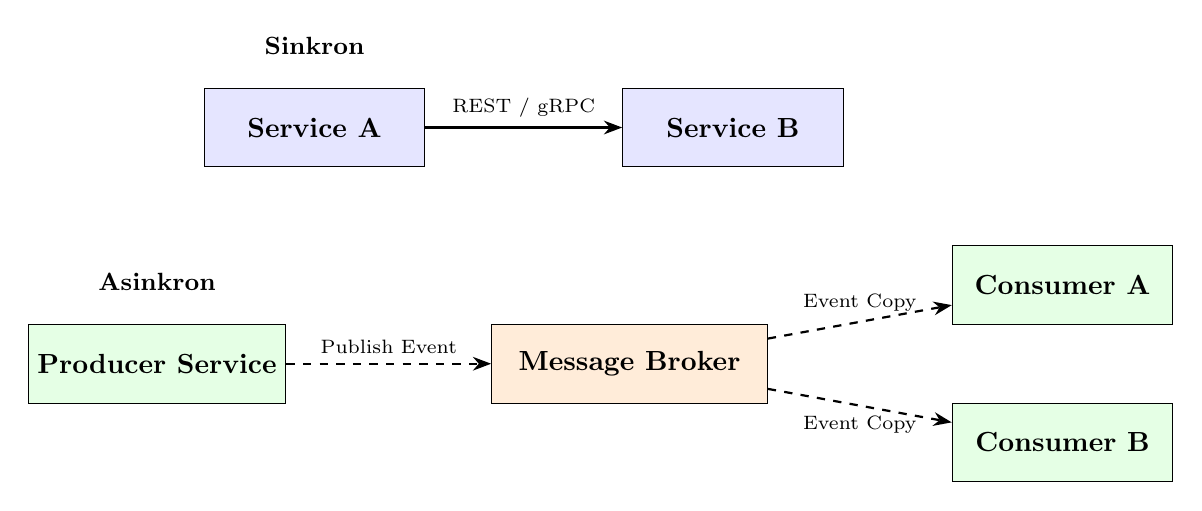
\begin{tikzpicture}[
			component/.style={draw, fill=blue!10, minimum width=2.8cm, minimum height=1cm, font=\bfseries, align=center},
			service/.style={draw, fill=green!10, minimum width=2.8cm, minimum height=1cm, font=\bfseries, align=center},
			broker/.style={draw, fill=orange!15, minimum width=3.5cm, minimum height=1cm, font=\bfseries, align=center},
			conn/.style={->, thick, >=Stealth},
			async/.style={->, thick, dashed, >=Stealth},
			label/.style={font=\scriptsize},
			node distance=1.4cm and 2.5cm
			]
			% Sinkron - REST/gRPC
			\node[component] (client1) at (0,0) {Service A};
			\node[component, right=of client1] (service1) {Service B};
			\draw[conn] (client1) -- node[above, label] {REST / gRPC} (service1);
			\node[font=\small, above=0.3cm of client1, align=center] {\textbf{Sinkron}};
			
			% Asinkron - Event-driven
			\node[service] (producer) at (-2,-3) {Producer Service};
			\node[broker] (broker) at (4,-3) {Message Broker};
			\node[service] (consumer1) at (9.5,-2) {Consumer A};
			\node[service] (consumer2) at (9.5,-4) {Consumer B};
			\draw[async] (producer) -- node[above, label] {Publish Event} (broker);
			\draw[async] (broker) -- node[above, label] {Event Copy} (consumer1);
			\draw[async] (broker) -- node[below, label] {Event Copy} (consumer2);
			\node[font=\small, above=0.3cm of producer, align=center] {\textbf{Asinkron}};
		\end{tikzpicture}
	\end{figure}
\end{frame}

\subsection{Komunikasi Sync: REST dan gRPC}

\begin{frame}[fragile]{Komunikasi Sync: REST dan gRPC}
	\vspace{20pt}
	\begin{columns}[T]
		\column{0.5\textwidth}
		\textbf{REST (HTTP/1.1)}
		\begin{itemize}
			\item API populer, berbasis HTTP
			\item Format umum: JSON, XML
			\item Mudah diintegrasi dan debug
			\item Alat: Swagger, Postman, OpenAPI
			\item Kurang efisien untuk real-time
		\end{itemize}
		
		\textbf{Penggunaan}
		\begin{itemize}
			\item Komunikasi antar tim
			\item Integrasi publik/lintas platform
			\item Cocok untuk permintaan data
		\end{itemize}
		
		\column{0.5\textwidth}
		\textbf{gRPC (HTTP/2)}
		\begin{itemize}
			\item Performa tinggi, pakai Protocol Buffers
			\item Mendukung streaming dan multiplexing
			\item Komunikasi efisien dan low-latency
			\item Sulit dibaca manusia secara langsung
		\end{itemize}
		
		\textbf{Penggunaan}
		\begin{itemize}
			\item Komunikasi internal antarlayanan
			\item Cocok untuk IoT, ML, gaming backend
			\item Real-time, skenario intensif
		\end{itemize}
	\end{columns}
	\vspace{5pt}
	\scriptsize
	\textit{Gunakan circuit breaker, timeout, retry untuk cegah efek domino saat layanan gagal.}
\end{frame}

\subsection{Komunikasi Async: Event-Driven Messaging}

\begin{frame}[fragile]{Komunikasi Async: Event-Driven Messaging}
	\vspace{20pt}
	\begin{columns}[T]
		\column{0.5\textwidth}
		\textbf{Konsep Utama}
		\begin{itemize}
			\item Tidak tunggu respons — non-blocking
			\item Event dikirim via broker (Kafka, RabbitMQ, dsb.)
			\item Cocok untuk sistem terdistribusi \& skalabel
		\end{itemize}
		
		\textbf{Polanya}
		\begin{itemize}
			\item \textbf{Publish/Subscribe}: semua subscriber menerima event
			\item \textbf{Message Queue}: satu konsumer tiap pesan (job worker)
		\end{itemize}
		
		\column{0.5\textwidth}
		\textbf{Keunggulan}
		\begin{itemize}
			\item Loose coupling dan fleksibel
			\item Pemrosesan paralel \& resilient
			\item Cocok untuk streaming data dan beban tinggi
		\end{itemize}
		
		\textbf{Tantangan}
		\begin{itemize}
			\item Sulit observability dan tracing
			\item Perlu retry, idempoten, dan penanganan duplikasi
			\item Konsistensi data terdistribusi jadi isu
		\end{itemize}
	\end{columns}
	\vspace{5pt}
	\scriptsize
	\textit{Sering dikombinasikan dengan REST/gRPC untuk arsitektur yang tangguh dan adaptif.}
\end{frame}



\subsection{Perbandingan dan Trade-Off}

\begin{frame}[fragile]{Karakteristik dan Trade-Off}
	\vspace{20pt}
	\begin{columns}[T]
		\column{0.5\textwidth}
		\textbf{Komunikasi Sinkron}
		\begin{itemize}
			\item Model sederhana, linier
			\item Hasil langsung (request/response)
			\item Cocok untuk validasi dan interaksi
			\item Mudah di-debug, alur deterministik
			\item Risiko cascading failure tinggi
			\item Sulit diskalakan elastis
		\end{itemize}
		
		\column{0.5\textwidth}
		\textbf{Komunikasi Asinkron}
		\begin{itemize}
			\item Event-driven, non-blocking
			\item Layanan loosely coupled
			\item Cocok untuk pemrosesan latar \& paralel
			\item Skalabilitas tinggi
			\item Kompleksitas observabilitas tinggi
			\item Perlu strategi retry, idempoten, replay
		\end{itemize}
	\end{columns}
	
	\vspace{10pt}
	\scriptsize
	\textit{Pendekatan hibrid banyak digunakan: sinkron untuk operasi kritis, asinkron untuk proses non-kritis.}
\end{frame}

\begin{frame}[fragile]{Tabel Perbandingan Sinkron vs Asinkron}
	\vspace{20pt}
	\scriptsize
	\arrayrulecolor{black}
	\setlength{\arrayrulewidth}{0.4pt} % garis tepi hitam tipis eksplisit
	\begin{table}[H]
		\centering
		\renewcommand{\arraystretch}{1.3}
		\begin{tabular}{|p{0.2\textwidth}|p{0.36\textwidth}|p{0.36\textwidth}|}
			\rowcolor{gray!25}
			\hline
			\textbf{Aspek} & \textbf{Sinkron (REST/gRPC)} & \textbf{Asinkron (Messaging)} \\
			\hline
			Model Komunikasi & Request/Response langsung & Event-based, tidak menunggu respons \\
			\hline
			Keterkaitan Layanan & Tight coupling & Loose coupling \\
			\hline
			Ketergantungan Respons & Harus tersedia saat itu juga & Bisa diproses kemudian \\
			\hline
			Skalabilitas & Terbatas oleh layanan terlemah & Tinggi, mendukung paralelisme \\
			\hline
			Kompleksitas Debugging & Rendah, alur linier & Tinggi, alur tidak deterministik \\
			\hline
			Kesesuaian Penggunaan & Validasi langsung, interaksi user & Proses latar, integrasi, notifikasi \\
			\hline
		\end{tabular}
	\end{table}
\end{frame}



\section{Komponen}

\begin{frame}[fragile]{Komponen Infrastruktur Mikroservis}
	\vspace{20pt}
	\begin{columns}[T]
		\column{0.5\textwidth}
		\textbf{API Gateway}
		\begin{itemize}
			\item Titik masuk semua request eksternal
			\item Tangani autentikasi, rate limiting, transformasi
			\item Contoh: Kong, NGINX, Apigee
		\end{itemize}
		
		\textbf{Service Registry \& Discovery}
		\begin{itemize}
			\item Daftar layanan aktif \& lokasi runtime
			\item Client/server-side discovery
			\item Contoh: Eureka, Consul, Zookeeper
		\end{itemize}
		
		\column{0.5\textwidth}
		\textbf{Configuration Server}
		\begin{itemize}
			\item Konfigurasi eksternal terpusat
			\item Dukungan multi-lingkungan
			\item Contoh: Spring Cloud Config Server
		\end{itemize}
		
		\textbf{Service Mesh (Opsional)}
		\begin{itemize}
			\item Kelola komunikasi via sidecar proxy
			\item Observabilitas, TLS, retry, circuit breaking
			\item Contoh: Istio, Linkerd, Kuma
		\end{itemize}
	\end{columns}
\end{frame}

\section{Microservices Patterns}


\subsection{Decomposition by Business Capability}
\begin{frame}[fragile]{Decomposition by Business Capability}
	\vspace{10pt}
	\begin{columns}[T]
		\column{0.5\textwidth}
		Pola ini memisahkan layanan berdasarkan kapabilitas bisnis, bukan lapisan teknis. 
		Setiap layanan bertanggung jawab atas satu domain fungsional yang utuh, seperti:
		\begin{itemize}
			\item \textbf{Order Service}
			\item \textbf{Payment Service}
			\item \textbf{Inventory Service}
		\end{itemize}
		Pendekatan ini mendukung \textit{bounded context} (DDD) sehingga:
		\begin{itemize}
			\item Struktur sistem lebih modular
			\item Tim dapat bekerja terdistribusi
			\item API dan logika bisnis lebih fokus domain
		\end{itemize}
		
		\column{0.5\textwidth}
		\begin{figure}
			\centering
			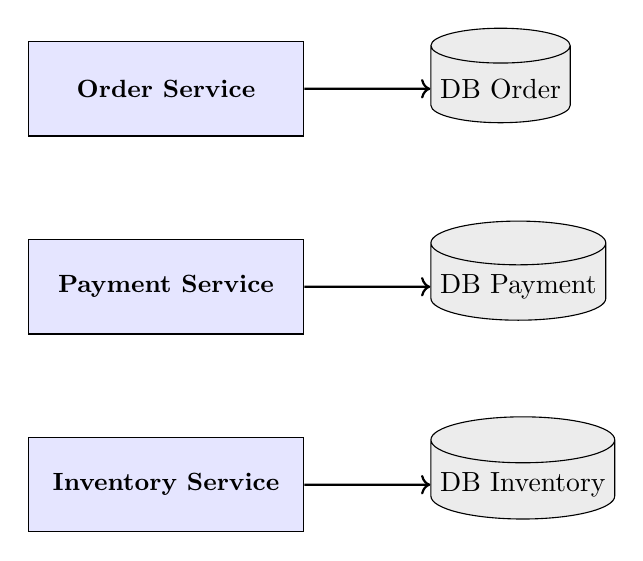
\begin{tikzpicture}[
				service/.style={draw, fill=blue!10, minimum width=3.5cm, minimum height=1.2cm, font=\small\bfseries, align=center},
				db/.style={draw, cylinder, shape border rotate=90, aspect=0.25, minimum height=1.2cm, minimum width=1.2cm, fill=gray!15},
				conn/.style={->, thick},
				node distance=1.3cm and 1.6cm
				]
				\node[service] (order) {Order Service};
				\node[service, below=of order] (payment) {Payment Service};
				\node[service, below=of payment] (inventory) {Inventory Service};
				
				\node[db, right=of order] (db1) {DB Order};
				\node[db, right=of payment] (db2) {DB Payment};
				\node[db, right=of inventory] (db3) {DB Inventory};
				
				\draw[conn] (order) -- (db1);
				\draw[conn] (payment) -- (db2);
				\draw[conn] (inventory) -- (db3);
			\end{tikzpicture}
		\end{figure}
	\end{columns}
\end{frame}

\subsection{Database per Service}
\begin{frame}[fragile]{Database per Service}
	\vspace{20pt}
	\begin{columns}[T]
		\column{0.45\textwidth}
		\begin{figure}
			\centering
			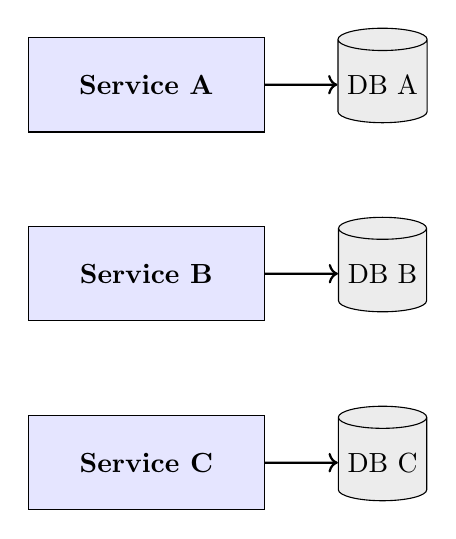
\begin{tikzpicture}[
				service/.style={draw, fill=blue!10, minimum width=3cm, minimum height=1.2cm, font=\bfseries},
				db/.style={draw, cylinder, shape border rotate=90, aspect=0.25, minimum height=1.2cm, minimum width=1cm, fill=gray!15},
				conn/.style={->, thick}
				]
				\node[service] (svc1) at (0,0) {Service A};
				\node[service] (svc2) at (0,-2.4) {Service B};
				\node[service] (svc3) at (0,-4.8) {Service C};
				
				\node[db] (db1) at (3,0) {DB A};
				\node[db] (db2) at (3,-2.4) {DB B};
				\node[db] (db3) at (3,-4.8) {DB C};
				
				\draw[conn] (svc1) -- (db1);
				\draw[conn] (svc2) -- (db2);
				\draw[conn] (svc3) -- (db3);
			\end{tikzpicture}
		\end{figure}
		
		\column{0.55\textwidth}
		\vspace{5pt}
		\textbf{Database per Service} \\
		\vspace{6pt}
		Pola ini memastikan setiap layanan memiliki database terpisah, mendorong:
		\begin{itemize}
			\item Isolasi data antar layanan
			\item Kebebasan memilih teknologi penyimpanan
			\item Penghindaran \textit{tight coupling} di level database
		\end{itemize}
	\end{columns}
\end{frame}

\subsection{Circuit Breaker}
\begin{frame}[fragile]{Circuit Breaker Pattern}
	\vspace{20pt}
	\begin{center}
		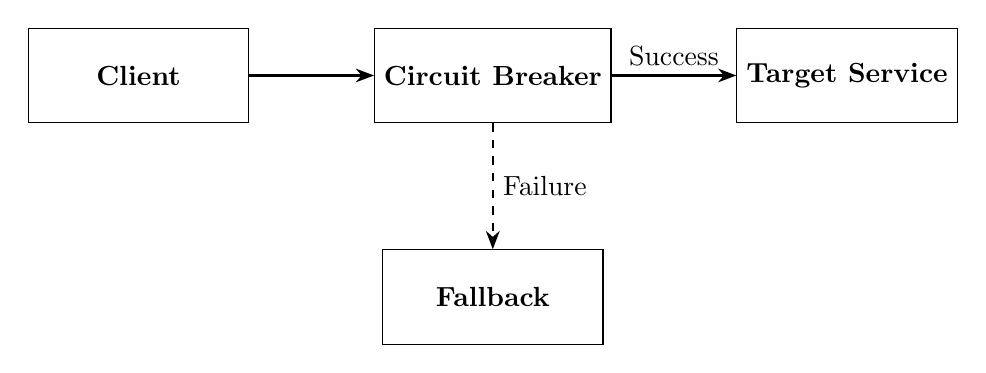
\begin{tikzpicture}[
			component/.style={draw, minimum width=2.8cm, minimum height=1.2cm, font=\bfseries, align=center},
			conn/.style={->, thick},
			alt/.style={dashed, thick, ->},
			>=Stealth
			]
			\node[component] (client) at (0, 0) {Client};
			\node[component] (cb) at (4.5, 0) {Circuit Breaker};
			\node[component] (service) at (9, 0) {Target Service};
			\node[component, below=1.6cm of cb] (fallback) {Fallback};
			
			\draw[conn] (client) -- (cb);
			\draw[conn] (cb) -- node[above]{Success} (service);
			\draw[alt] (cb) -- node[right]{Failure} (fallback);
		\end{tikzpicture}
	\end{center}
	
	\vspace{12pt}
	\small
	Pola ini memutus permintaan ke layanan gagal untuk mencegah cascading failure. Terdiri dari tiga status: \textbf{Closed} (berfungsi normal), \textbf{Open} (putus sementara), dan \textbf{Half-Open} (uji coba pulih). 
\end{frame}

\subsection{Saga Pattern}
\begin{frame}[fragile]{Saga Pattern (Orchestration)}
	\vspace{20pt}
	\begin{columns}[T]
		\column{0.74\textwidth}
		\begin{figure}
			\centering
			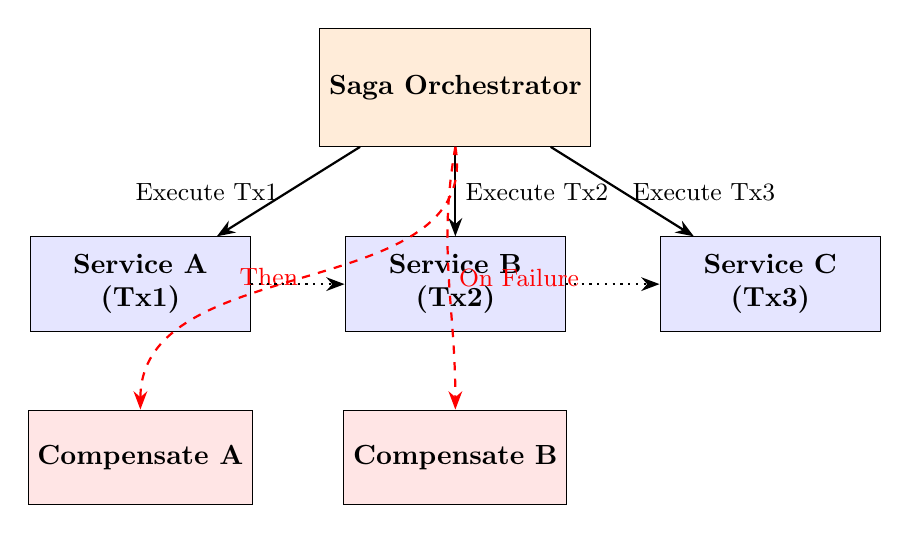
\begin{tikzpicture}[
				service/.style={draw, minimum width=2.8cm, minimum height=1.2cm, font=\bfseries, align=center, fill=blue!10},
				orchestrator/.style={draw, minimum width=3cm, minimum height=1.5cm, font=\bfseries, align=center, fill=orange!15},
				conn/.style={->, thick, >=Stealth},
				rollback/.style={->, thick, dashed, red, >=Stealth},
				flow/.style={->, thick, dotted, >=Stealth}
				]
				
				% Nodes
				\node[orchestrator] (orchestrator) at (0, 2.5) {Saga Orchestrator};
				
				\node[service] (service1) at (-4, 0) {Service A \\ (Tx1)};
				\node[service] (service2) at (0, 0) {Service B \\ (Tx2)};
				\node[service] (service3) at (4, 0) {Service C \\ (Tx3)};
				
				% Compensation handlers
				\node[service, fill=red!10] (comp1) at (-4, -2.2) {Compensate A};
				\node[service, fill=red!10] (comp2) at (0, -2.2) {Compensate B};
				
				% Connections from orchestrator to services
				\draw[conn] (orchestrator) -- node[left, font=\small] {Execute Tx1} (service1);
				\draw[conn] (orchestrator) -- node[right, font=\small] {Execute Tx2} (service2);
				\draw[conn] (orchestrator) -- node[right, font=\small] {Execute Tx3} (service3);
				
				% Compensation arrows (rollback)
				\draw[rollback] (orchestrator.south) to[out=-100,in=90] node[right, font=\small] {On Failure} (comp2.north);
				\draw[rollback] (orchestrator.south) to[out=-80,in=90] node[left, font=\small] {Then} (comp1.north);
				
				% Logical dotted flow
				\draw[flow] (service1) -- (service2);
				\draw[flow] (service2) -- (service3);
			\end{tikzpicture}
		\end{figure}
		
		\column{0.26\textwidth}
		\small
		\textbf{Saga Pattern} membagi proses bisnis menjadi transaksi lokal terpisah. \textit{Orchestrator} mengatur urutan dan eksekusi antar layanan. Jika gagal, aksi kompensasi dijalankan untuk menjaga konsistensi. Dua pendekatan umum: \textit{choreography} dan \textit{orchestration}.
	\end{columns}
\end{frame}

\subsection{Sidecar}
\begin{frame}[fragile]{Sidecar Pattern}
	\vspace{10pt}
	\begin{center}
		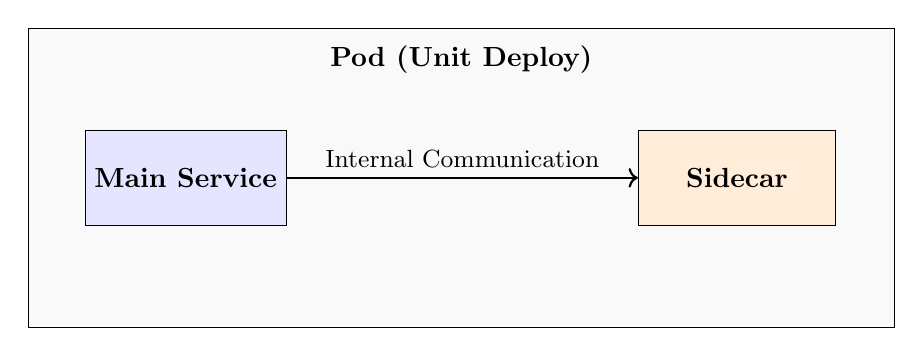
\begin{tikzpicture}[
			box/.style={draw, minimum height=3.8cm, minimum width=11cm, fill=gray!5},
			service/.style={draw, fill=blue!10, minimum width=2.5cm, minimum height=1.2cm, font=\bfseries, align=center},
			sidecar/.style={draw, fill=orange!15, minimum width=2.5cm, minimum height=1.2cm, font=\bfseries, align=center},
			label/.style={font=\small\bfseries}
			]
			
			% Pod box with label above
			\node[box] (pod) {};
			\node[font=\bfseries, above=-.7cm of pod.north] {Pod (Unit Deploy)};
			
			% Inside Pod: Main Service and Sidecar
			\node[service] (main) at (-3.5, 0) {Main Service};
			\node[sidecar] (sc) at (3.5, 0) {Sidecar};
			
			% Internal arrow
			\draw[->, thick] (main) -- node[above, font=\small] {Internal Communication} (sc);
			
		\end{tikzpicture}
	\end{center}
	
	\vspace{10pt}
	\small
	Pola \textbf{Sidecar} menempatkan komponen tambahan (seperti proxy, logger, config agent) berdampingan dengan layanan utama dalam satu unit deploy. Fungsi infrastruktur dikelola terpisah, meningkatkan modularitas tanpa membebani kode utama.
\end{frame}

\section{Teknologi Pendukung}
\begin{frame}[fragile]{Teknologi Pendukung Mikroservis}
	\vspace{20pt}
	\small
	\begin{columns}[T]
		\column{0.5\textwidth}
		\textbf{Docker \& Kubernetes}
		
		\begin{itemize}
			\item \textbf{Docker:} Containerisasi layanan mikroservis agar terisolasi dan portable.
			\item \textbf{Kubernetes:} Orkestrasi container: scaling, deployment, service discovery.
		\end{itemize}
		
		\vspace{5pt}
		\textbf{Framework Pengembangan}
		\begin{itemize}
			\item \textbf{Spring Boot (Java):} Integrasi Spring Cloud, REST, konfigurasi sentral.
			\item \textbf{Express.js (Node.js):} REST API cepat dan minimalis.
			\item \textbf{FastAPI (Python):} Async, validasi otomatis, dokumentasi OpenAPI.
		\end{itemize}
		
		\column{0.5\textwidth}
		\textbf{Observability: Prometheus \& Grafana}
		
		\begin{itemize}
			\item \textbf{Prometheus:} Time-series DB, alerting, query PromQL.
			\item \textbf{Grafana:} Visualisasi dashboard interaktif dan alert metrics.
		\end{itemize}
		
		\vspace{5pt}
		\textbf{Service Mesh: Istio \& Linkerd}
		\begin{itemize}
			\item \textbf{Istio:} Envoy proxy, telemetry, keamanan, tracing (Jaeger/Zipkin).
			\item \textbf{Linkerd:} Lightweight, setup sederhana, efisien untuk pemula.
		\end{itemize}
	\end{columns}
\end{frame}

\section{Best Practices}
\begin{frame}[fragile]{Best Practices dalam Mikroservis}
	\vspace{20pt}
	\small
	\begin{columns}[T]
		\column{0.5\textwidth}
		\textbf{Bounded Context dan DDD}
		\begin{itemize}
			\item Setiap layanan memiliki domain yang jelas (bounded context).
			\item Hindari campur logika atau model antar domain.
		\end{itemize}
		
		\vspace{5pt}
		\textbf{Distributed Logging \& Monitoring}
		\begin{itemize}
			\item Gunakan trace ID dan service name dalam log.
			\item Prometheus + Grafana untuk metrik; Jaeger/Zipkin untuk tracing.
		\end{itemize}
		
		\column{0.5\textwidth}
		\textbf{Contract Testing antar Layanan}
		\begin{itemize}
			\item Pastikan provider dan consumer mengikuti kontrak API.
			\item Deteksi dini perubahan yang merusak integrasi.
		\end{itemize}
		
		\vspace{5pt}
		\textbf{CI/CD dan Otomasi Deployment}
		\begin{itemize}
			\item Build dan test tiap layanan secara mandiri.
			\item Gunakan GitHub Actions, GitLab CI/CD, Jenkins, ArgoCD, Helm.
		\end{itemize}
	\end{columns}
\end{frame}

\section{Contoh Implementasi Sederhana}
\begin{frame}[fragile]{Contoh Implementasi Sederhana}
	\vspace{20pt}
	\small
	Contoh aplikasi dapat dilihat pada \textbf{Bab 2: Container}. Aplikasi \textit{microservices} ini terdiri dari empat layanan terpisah yang dikemas dalam \textit{Docker container} dan berkomunikasi melalui jaringan virtual bersama.
	
	\vspace{10pt}
	\begin{itemize}
		\item \texttt{Employee Service}: menangani permintaan data karyawan.
		\item \texttt{Performance Service}: memproses data performa berdasarkan ID.
		\item Keduanya menggunakan \texttt{MariaDB} untuk penyimpanan data.
		\item Antarmuka \texttt{phpMyAdmin} disediakan untuk akses basis data.
	\end{itemize}
	
	\vspace{10pt}
	Setiap layanan dapat dikembangkan, diuji, dan di-deploy secara independen dengan memanfaatkan isolasi dan portabilitas container. Hasilnya adalah sistem \textit{microservices} yang ringan, modular, dan mudah dipelihara.
\end{frame}

\section{Kesimpulan}
\begin{frame}[fragile]{Kesimpulan}
	\vspace{20pt}
	\small
	\begin{columns}[T]
		\column{0.48\textwidth}
		\textbf{Manfaat Mikroservis}
		\begin{itemize}
			\item Layanan modular dan otonom
			\item Skalabilitas horizontal
			\item Rilis cepat dan fleksibel
			\item Pilihan teknologi bebas per domain
		\end{itemize}
		
		\vspace{10pt}
		\textbf{Tantangan Umum}
		\begin{itemize}
			\item Kompleksitas komunikasi
			\item Konsistensi data terdistribusi
			\item Observabilitas dan debugging
		\end{itemize}
		
		\column{0.48\textwidth}
		\textbf{Kunci Keberhasilan}
		\begin{itemize}
			\item Desain \textit{bounded context}
			\item Contract testing antar layanan
			\item Otomasi CI/CD dan versioning
			\item Observabilitas sejak awal
		\end{itemize}
		
		\vspace{10pt}
		\textbf{Teknologi Pendukung}
		\begin{itemize}
			\item Docker, Kubernetes
			\item Prometheus, Grafana
			\item Spring Boot, Micronaut
		\end{itemize}
	\end{columns}
\vspace{10pt}
	\textit{Mikroservis efektif untuk sistem besar yang adaptif dan siap tumbuh.}
\end{frame}


\end{document}
